\section{Statische Analyse}
Die statische Analyse beschäftigt sich mit der Untersuchung der Malware, ohne diese auszuführen. Dies geschieht meist über Tools, welche die im Binary enthaltenen Informationen auslesen. Im folgenden werden verschiedene Methoden aufgezeigt, um die Malware statisch zu analysieren, ohne das Gastsystem einem Risiko zu unterziehen.

\subsection{Identifikation des Samples}
Zu aller erst wird das Zip-File aus der E-Mail gesichert und ein Hash erstellt, um das Sample in Zukunft auch unter einem anderen Namen identifizieren zu können. Der Hash wurde hier über die Software \textit{winMD5Free}\footnote{\url{http://winmd5.com/}} in der Version 1.20 genutzt. Alternativ hätte man unter Linux das Tool \textit{md5sum} nutzen können 
\begin{lstlisting}
ups_webtracking_1S63A0003659818362.zip
	--> 81397589ad7bf0a7faecf977644b1486
\end{lstlisting}
Die Datei wird im folgenden Text kurz \textit{8139} genannt. Um zu verifizieren, dass es sich bei der Datei \textit{8139} wirklich um ein Archiv handelt, wendet man in einem \textit{Linux}-System das \textit{File}-Kommando an. Wie in der Abbildung \ref{img:FileAufZip} zu sehen ist, bestätigt das \textit{File}-Kommando den Verdacht, dass es sich hier um ein Archiv handelt.
\begin{figure}[htbp]
	\centering
	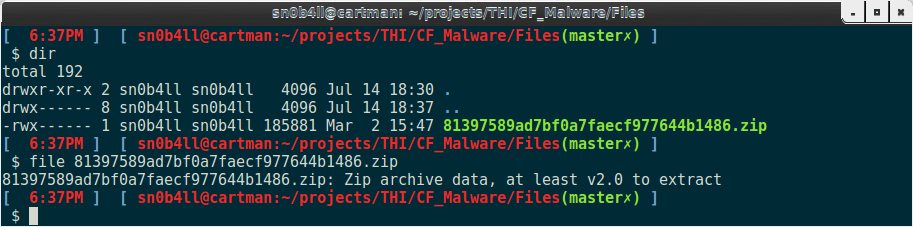
\includegraphics[width=\textwidth]{bilder/statischeAnalyse/fileAufZip.png}
	\caption{Anwendung des File-Kommandos auf die Datei \textit{8139}}
	\label{img:FileAufZip}
\end{figure}
Das File-Kommando identifiziert Dateien anhand derer Header und gibt somit meist einen verlässlichen ersten Eindruck, von welchem Typ die Datei ist. In anderen Gebieten, wie zum Beispiel der Steganographie, sollte man sich jedoch nicht uneingeschränkt darauf verlassen, sondern die Datei manuell untersuchen.
	
Da nun klar ist, dass es sich bei der Datei \textit{8139} wirklich um ein Archiv handelt, kann dieses nun entpackt werden. Hier wurde \textit{7Zip}\footnote{\url{http://www.7-zip.de/}} unter Windows verwendet. Alternativ hätte man hier das \textit{Unzip}-Kommando\footnote{\url{http://www.info-zip.org/mans/unzip.html}} unter Linux nutzen können.
	
Als Ergebnis bekommt man eine Datei mit einem zur Spam-Mail passenden Namen. Von der Datei wird wiederum der Hash (MD5) entnommen.
\begin{lstlisting}
ups_webtracking_1S63[...]62_0003947_de_2015_02_tracknum_09234728.exe
	--> f113cf383214f2788876d27d644ab432	
\end{lstlisting}
Die Datei wird im Folgenden unter dem Namen \textit{f113} geführt. Aus der Endung \textit{.exe} lässt sich auf eine ausführbare Windows-Datei schließen. Die Datei \textit{f113} wird nun ebenfalls mit dem \textit{File}-Kommando untersucht, welches den Verdacht bestätigt (Abbildung \ref{img:FileAuff113}).

\begin{figure}[htbp]
	\centering
	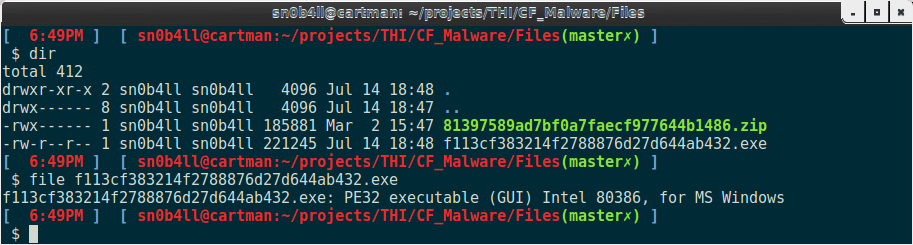
\includegraphics[width=\textwidth]{bilder/statischeAnalyse/fileAuff113.png}
	\caption{Anwendung des File-Kommandos auf die Datei \textit{f113}}
	\label{img:FileAuff113}
\end{figure}

\subsection{Virustotal}
\label{ref:statAnVirustotal}
Im Anschluss kann das Sample \textit{f113} auf \textit{Virustotal} (siehe Sektion \ref{ref:ToolsVirustotal}) hochgeladen werden. Das Ergebnis ist, dass bereits 44 von 56 Virenscannern das Sample erkennen. Als Malware-Familie (nach \textit{NOD32}) wird \textit{Win32/Emotet.AD} angegeben. Ebenso werden alternative Dateinamen wie 
\begin{itemize}
	\item Telekom\_Rechnung\_2015\_02\_de\_04349\_AIEO\_POP\_MAIL\_W5\_5[...]H.exe
	\item dhl\_paket\_de\_003407293054131348371\_02\_2015\_HD\_38300\_J[...]MAIL.exe
\end{itemize} angegeben. Daraus lässt sich schließen, dass die Malware bereits in anderen Spam-Angriffen Anwendung fand. Es werden ebenfalls weiterführende Informationen zum Sample geliefert, welche jedoch im Folgenden über lokale Tools erarbeitet werden. Dies hat den Hintergrund, dass, falls man Opfer eines gezielten Angriffs ist, das Sample nicht umgehend bei Virustotal veröffentlicht werden sollte. Ein Angreifer könnte regelmäßig prüfen, ob das Sample Virustotal bereits bekannt ist. Ist das Sample online, weiß der Angreifer, dass man einen ersten Verdachtsmoment hat und beginnt eventuell damit, seine Spuren zu verwischen.

\subsection{Resource Hacker}
\label{ref:StatAnResourceHacker}
Nun findet das \textit{Resource Hacker} (siehe Abschnitt \ref{ResourceHacker}) Anwendung. Hierzu öffnet man die Anwendung und lädt anschließend über \textit{File} $\rightarrow$ \textit{Open} die Datei \textit{f113}.
\begin{figure}[htbp]
	\centering
	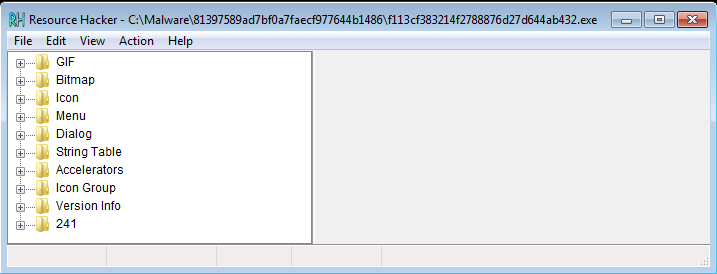
\includegraphics[width=\textwidth]{bilder/statischeAnalyse/ResourceHacker.png}
	\caption{Anwendung des Tools \textit{Resource Hacker} auf die Datei \textit{f113}}
	\label{img:FileAufZip}
\end{figure}
In den jeweiligen Kategorien lassen sich verschiedene Informationen darstellen. Insbesondere drei Informationen fallen bei der Analyse des Files \textit{f113} auf.
\begin{description}
	\item[1. Version Info:]Im Feld \textit{Version Info} wird die Versions-Information des bekannten First-Person-Shooters \textit{Half-Life} von \textit{Valve}\footnote{\url{http://store.steampowered.com/app/70}} verwendet. Der volle Text ist im Anhang unter \ref{ref:versionInfo} zu finden. Diese Maßnahme wird vermutlich verwendet, um die Malware zu tarnen. Durch die kleinste Veränderung von Inhalten wird der Hash der Datei verändert, wodurch primitive Vergleiche das Sample nicht mehr erkennen würden. Zudem können Anti-Viren-Herstellter schlecht den Text als Pattern hinterlegen, da sonst in Zukunft die ausführbare Datei des Spiels \textit{Half-Life} als Malware erkannt werden könnte. Dies wäre ein sogenanntes \textit{False-Positive}, also eine Datei, welche keine Malware ist aber als solche erkannt wird. Im Allgemeinen versuchen Anti-Viren-Hersteller dies zu vermeiden, da sonst die Akzeptanz der Produkte sinkt.
	
	\item[2. Icon:] Im Feld \textit{Icon} kann das in der Abbildung \ref{img:Iconf113} gezeigte Icon gefunden werden. Es zeigt das Logo des \textit{Akrobat Readers}\footnote{\url{https://get.adobe.com/de/reader/otherversions/}}. Es wurde vermutlich gewählt, um den Nutzer den Eindruck zu vermitteln, es würde sich um eine \textit{PDF}-Datei handeln, welche zumeist mit dem \textit{Akrobat Reader} geöffnet werden. Durch die weite Bekanntheit des \textit{Akrobat Readers} erreichen die Malware-Ersteller so eine höhere Quote der Fälle, in welchen die Malware geöffnet wird.
	
\begin{figure}[htbp]
	\centering
	
\includegraphics[scale=1]{bilder/statischeAnalyse/Icon.png}
	\caption{Icon der Datei \textit{f113}}
	\label{img:Iconf113}
\end{figure}

	\item[3. Menü-Bestandteile:] In den Feldern \textit{Bitmap}, \textit{Menu} und \textit{Dialog} können Bestandteile eines Menüs gefunden werden. Die Abbildung \ref{img:Bitmapf113} zeigt das unter \textit{Bitmap} zu findende Bild, welches eine herkömmliche Werkzeugleiste eines Programms zeigt. Unter dem Punkt \textit{Menu} kann zudem ein volles Menü mit asiatischen Schriftzeichen gefunden werden. \textit{Resource Hacker} erlaubt es hier, sich das Menü, wie es im Programm eingebetet wäre, zu inspizieren. Es zeigt sich ein normales Menü, aus dem man, auch ohne die Schriftzeichen zu verstehen, normale Felder wie Öffnen, Speichern oder Schließen ableiten kann (siehe Abbildung \ref{img:Menuf113}). Die Beweggründe, warum das Menü enthalten ist, können unterschiedlich sein. Es könnte direkt vom Programm stammen, sodass man zum Beispiel durch eine bestimmte Eingabe eine Menü öffnen kann. Alternativ kann es auch nur ein weiteres Element der Malware sein, um das Sample schwer von Pattern erfassbar zu machen. Eine andere Alternative wäre, dass die Malware-Ersteller hier Analysten zu falschen Schlussfolgerungen bringen wollen, zum Beispiel, dass die Malware aus dem asiatischen Raum stammt. Daher sollte mit dieser Information sehr behutsam umgegangen werden und die Thesen später bei einem tieferen Wissen nochmals geprüft werden. Zudem ist unter dem Feld \textit{Dialog} ein kleiner Dialog zu finden, welcher in der Abbildung \ref{img:Dialogf113} dargestellt ist.
	
	\begin{figure}[htbp]
		\centering
		
\includegraphics[scale=1]{bilder/statischeAnalyse/Bitmap.png}
		\caption{Enthaltenes Bitmap der Datei \textit{f113}}
		\label{img:Bitmapf113}
	\end{figure}
	\begin{figure}[htbp]
		\centering
		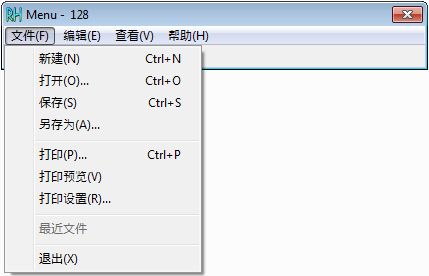
\includegraphics[scale=0.5]{bilder/statischeAnalyse/Menu.png}
		\caption{Enthaltenes Menü der Datei \textit{f113}}
		\label{img:Menuf113}
	\end{figure}
	\begin{figure}[htbp]
		\centering
		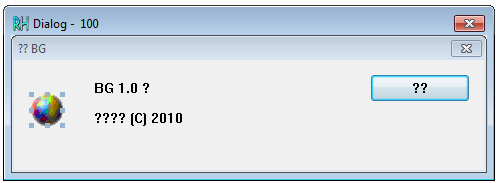
\includegraphics[scale=0.5]{bilder/statischeAnalyse/Dialog.png}
		\caption{Enthaltener Dialog der Datei \textit{f113}}
		\label{img:Dialogf113}
	\end{figure}
\end{description}

\subsection{Dependency Walker}
\label{ref:DependencyWalker}
Als nächstes wird die Datei \textit{f113} mit der Software \textit{Dependency Walker} (siehe Beschreibung \ref{ref:dependencyWalker}) untersucht. Dazu öffnet man den Dependency Walker und öffnet über \textit{File} $\rightarrow$ \textit{Open} die Datei \textit{f113}. Daraufhin zeigt \textit{Dependency Walker} alle verwendeten \textit{DLLs}, sowie deren genutzte Funktionen an. Das Ergebnis ist im Anhang in der Abbildung \ref{img:depWalkerf113} zu sehen. Aus den aufgerufenen Funktionen der \textit{Kernel32.dll} kann man auf die Funktionsweise der Malware schließen. Die interessanten Funktionen sind im Folgenden aufgeführt:
\begin{description}
\item[CompareStringA:] Es wird ein String-Vergleich angestellt. Dies könnte in vielen Szenarien zum Einsatz kommen. Möglichkeiten wären hier ein Vergleich um zu erkennen, ob die Malware in einer VM ausgeführt wird oder ein einfacher Vergleich, in welchem Ordner sich die aktuell ausgeführte Datei befindet.

\item[CreateFileW:] Es wird eine Datei auf das Dateisystem geschrieben. Dies könnte zum Beispiel eine Datei sein, welche beim Systemstart ausgeführt wird.

\item[FindNextFileA:] Es wird nach einer Datei gesucht. Dies kann wiederum der Erkennung einer VM dienen, falls zum Beispiel nach einer bestimmten \textit{DLL} gesucht wird, welche nur von \textit{VMWare} (oder \textit{VirualBox}) verwendet wird.

\item[GetModuleFileNameW:] Es wird entweder der Pfad zu einem Modul oder, falls kein Parameter übergeben wurde, die Pfad zur ausgeführten Anwendung zurückgegeben. Dies könnte zusammen mit \textit{CompareStringA} dazu genutzt werden, die aktuelle Position der Datei \textit{f113} abzufragen und ausgehend davon verschiedene Aktionen auszuführen.

\item[GetModuleHandleW:] Über diese Funktion kann auf eine bereits geladene \textit{DLL} zugegriffen werden. Gelingt es der Malware eine \textit{DLL} in den Kontext zu laden, könnte diese damit benutzt werden.

\item[GetStartupInfoW:] Es wird der \textit{StartupInfo}-Vektor abgefragt. Dieser umfasst unter anderem den Rechnernamen, den Titel der Anwendung sowie andere Elemente des Environments.\footnote{\url{https://msdn.microsoft.com/en-us/library/windows/desktop/ms686331(v=vs.85).aspx}}

\item[HeapSize und VirtualAlloc:] \textit{HeapSize} gibt die aktuelle Größe des \textit{Heaps} an. \textit{VirtualAlloc} reserviert Speicherbereiche. Das Besondere an \textit{VirtualAlloc} ist, dass für die reservierten Speicherbereiche \textit{DEP} deaktiviert werden kann.\footnote{\url{http://0xdabbad00.com/2012/12/07/dep-data-execution-prevention-explanation/}} Dies könnte ein Hinweis dafür sein, dass die Malware versucht (eventuell dynamisch nachgeladenen) \textit{Shellcode} auszuführen. Die \textit{HeapSize} kann dazu eine wichtige Information sein (wird jedoch nicht unbedingt benötigt).
\end{description}

Ob durch die Malware alle festgestellten Funktionen ausgeführt werden, lässt sich in der statischen Analyse nur sehr schwer feststellen. Zudem kann der Ersteller der Malware zu jeder Zeit nicht wirklich benötigte Funktionen einschleusen, um die Analyse zu erschweren.
	
\subsection{PEView}
\label{ref:statAnPEView}
Als nächstes wird das Tool \textit{PEView} (siehe Beschreibung \ref{ref:PEView}) angewendet. Dazu wird \textit{PEView} gestartet und die Datei \textit{f113} ausgewählt. Daraufhin werden im \textit{PEView}-Fenster die verschiedenen Sektionen der ausführbaren Datei anzeigt, wie zu sehen in Abbildung \ref{img:PEViewf113}. Auffällig waren dabei:
\begin{description}
\item[SECTION .data:] Enthält den Text "Rocal AppWizard-Generated Application". Dieser Text wurde bereits in vielen anderen Malware-Samples gefunden\footnote{\url{https://www.google.de/search?q=Rocal+AppWizard}} und wird auch später noch in der Registry auftauchen (siehe Abschnitt \ref{ref:DynAnRegShot}).

\item[SECTION .rsrc:] Enthält den Text "PADDINGXPADDINGXPADDINGX" vielfach. Es lassen sich 2 Funktionen ableiten. Entweder wurde das Padding genutzt, um die ausführbare Datei auf eine korrekte (vom PE/COFF-Format geforderte) Länge zu strecken oder als Padding bei einem möglichen Exploit (siehe \textit{VirtualAlloc} in Sektion \ref{ref:DependencyWalker}).
\end{description}

\begin{figure}[htbp]
	\centering
	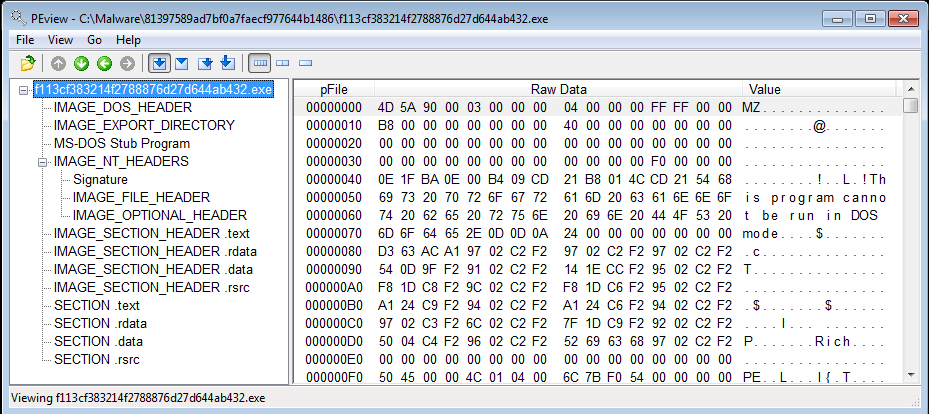
\includegraphics[scale=0.5]{bilder/statischeAnalyse/PEView.png}
	\caption{Aufruf der Datei \textit{f113} mit PEView}
	\label{img:PEViewf113}
\end{figure}
	
Leider liefert \textit{PEView} hier keine weiteren, neuen Informationen zur Datei \textit{f113}.

\subsection{IDA Pro Free}
Als letzten Schritt der statischen Analyse wird die Datei \textit{f113} mit dem Disassembler \textit{IDA PRO Free} (siehe Beschreibung \ref{ref:ToolIDA} untersucht. Dazu öffnen wir die Datei mit dem Programm. Wirft man einen Blick auf die enthaltenen Funktionen, so erkennt man viele, welche für graphische Oberflächen nützlich sind. Beispiele sind im Anhang in der Abbildung \ref{img:IDAFuncf113} aufgezeigt. Auffällig ist, dass viele der Funktionen anscheinend nicht aufgerufen werden oder nur im \textit{.rdata}-Segment verankert sind. Das diese Funktionen im Disassembler nicht genutzt werden, heißt jedoch nicht, dass das Programm in der Ausführung diese nicht dynamisch zur Laufzeit nutzt.
	
Die Analyse, beginnend mit der \textit{start}-Funktion, welche durch den Eintrittspunkt in das Programm ermittelt wird, ergibt folgendes:
\begin{description}
	\item[Funktion \textit{start}:] Es wird zu Anfang die Unterfunktion \textit{sub\_402718} aufgerufen, welche im weiteren Verlauf genauer analysiert wird. Nach dem Aufruf würde das Programm in Unterfunktion \textit{loc\_402C05} springen, in welcher ein neuer Thread erstellt wird. Danach endet das Programm.
	
	\item[Funktion \textit{sub\_402718}:] Die Funktion \textit{sub\_402718} ist wesentlich komplexer (siehe Abbildung \ref{img:IDASub402718f113}). Aktionen in der Klasse sind:
	\begin{enumerate}
		\item Es wird der Applikationstyp über \textit{set\_app\_type}\footnote{\url{https://msdn.microsoft.com/en-us/library/ff770596.aspx}} gesetzt.
		
		\item Anschließend werden einige Variablen und Vektoren initialisiert. Im Anschluss wird ein Sprung genommen, welcher dem Autor auf den ersten Blick nicht ersichtlich ist

\begin{lstlisting}
call    _initterm
add     esp, 24h
mov     eax, ds:_wcmdln
mov     esi, [eax]
cmp     esi, ebx
jnz     short contWithSub
\end{lstlisting}

	Fällt der Vergleich negativ aus, springt das Programm über eine kurze Unterroutine zurück in die \textit{start}-Funktion. Ist der Vergleich positiv, fährt die Funktion \textit{sub\_402718} fort und wird, wie sich später zeigt, nicht mehr in die start-Funktionen zurückkehren.
	
	\item Im Anschluss fährt das Programm über verschiedene Sub-Funktionen fort, welche vermutlich eine Schleife beinhalteten und weitere Variablen initialisiert (in der Abbildung \ref{img:IDASub402718f113} knapp nach der Hälfte zu sehen).
	
	\item Daraufhin wird die \textit{GetStartupInfoW} geladen und verglichen. Der Vergleich bestimmt jedoch nur, ob \textit{0Ah} oder der Wert an der Adresse\\ \textit{ebp+StartupInfo.wShowWindow} als Parameter für die nächste Funktion genutzt wird. Mit welchem Wert die \textit{StartupInfo} verglichen wird, ist leider nicht ersichtlich.
	
	\item Im weiteren Verlauf wird die Funktion \textit{GetModuleHandleW} aufgerufen, welche den \textit{Handle} auf ein Modul lädt. Welches dies genau ist, ist leider in \textit{IDA} nicht ersichtlich.
	
	\item Im Anschluss wird die (selbst-benannte) Funktion \textit{openWindow} aufgerufen, welche intern die Funktion \textit{AfxWinMain()} aufruft. Dadurch wird sehr wahrscheinlich ein Fenster erstellt. Die Funktion kehrt anschließend in die Funktion \textit{sub\_402718} zurück.
	
	\item Dort wird als letztes die Funktion \textit{exit} aufgerufen, welche das Programm beendet.
	\end{enumerate}
\end{description}

\begin{figure}[htbp]
	\centering
	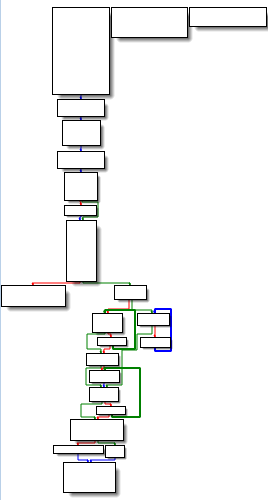
\includegraphics[scale=0.25]{bilder/statischeAnalyse/IDASub402718.png}
	\caption{Funktion sub\_402718 der Datei \textit{f113}, Ansicht in IDA Graphview}
	\label{img:IDASub402718f113}
\end{figure}

Anmerkung: Die statische Disassemblierung gibt eine grobe Einsicht in das Programm, kann aber niemals allen Sprüngen folgen. Es werden von Malware-Entwicklern oft Techniken genutzt, welche die statische Disassemblierung wesentlich erschweren (dynamisches Laden von Programmteilen, Verschlüsselung kritischer Abschnitte oder Ähnliches). Auch hier wurde sehr sicher nicht der volle Funktionsumfang erfasst, da der Thread nur mit wesentlich erhöhtem Aufwand nachverfolgt werden kann.

\subsection{Fazit zur statischen Analyse}
\label{ref:statAnFazit}
Die statische Analyse gab folgende Informationen
\begin{itemize}
\item Die Malware versucht das Opfer glauben zu lassen, sie wäre ein PDF. (siehe \ref{ref:StatAnResourceHacker})
\item Die Malware benutzt die Daten eines Videospiels als Versions-Informationen. (siehe \ref{ref:StatAnResourceHacker})
\item Die Malware beinhaltet Menü-Elemente. (siehe \ref{ref:StatAnResourceHacker})
\item Die Malware stellt Vergleiche an und erstellt eine oder mehrere Dateien. Ebenso führt sie eventuell Shellcode aus. (siehe \ref{ref:DependencyWalker})
\end{itemize}